\documentclass[11pt]{report}
\usepackage[utf8]{inputenc}
\usepackage[frenchb]{babel}
\usepackage[official]{eurosym}
\usepackage{amsmath}
\usepackage{graphicx}
%\DeclareGraphicsExtensions{.pdf,.png,.jpg,.eps}%
\begin{document}

%\includegraphics{elecshock}%

\title{Transmission d'electricité sans fil par le biais de systemes de tranfert d'energie inductive (IPTS)}
\author{Blaise Ribon, Léo Boudoin, Quentin Boyer}
\date{Décembre 2014}
\maketitle

\begin{abstract}
	Suite a l'experience menée en 2007 au MIT , nous savons qu'il est possible de transmettre de l'electricité à travers de moyennes distances, de l'ordre de 5m. Ce type de transmissions d'electricité pourrait simplifier les reseaux electriques domestiques étant donné le nombre de cables demandés par chaque appareil electronique, qui proliferent. Mais nous verrons que cette technologie et celles semblables se heurtent à des freins majeurs dans la pratique et que leur mise en place est assez complexe.
\end{abstract}

\tableofcontents

\chapter{Définition et Utilisation de l'electricité} %Titre a changer je pense%
\section{Historique de l'electricité}
	
\section{Avancées technologiques et Utilisation}

\chapter{Raisons de la transmission de l'electricité par des solutions non cablées} %Titre encore plus pété , Mais en fait on pourrait faire la demarche de projet sur la transimission d'electicté tout court en preseantant tour a tour les solutions cablées et non cablées , à voir%
\section{--TODO--}

\chapter{Les technologies de transmissions d'electricité : cablées et sans-fil} %A voir si on insiste autant sur les cables%
\section{Presentation des technologies présentes}
\subsection{Solution majoritaire actuelle : Les technoloogies cablées}
	La solution de transmission d'electricité la plus utilisée au monde est sans contestation possible le cable electrique , ceci étant du à un faible coût (jusqu'a 1\$ le métre) , son très haut rendement puisque celui ci avoisine les 100\% sur les distances courtes avec de faibles puissances. En plus d'etre simple , elle n'est pas lourde en terme d'installation puisque les cables peuvent etre facilement mis dans les murs à la constuction d'un nouveau batiment, etre mis dans des gaines si l'on veut en rajouter ensuite et plus simplement on peut utiliser le systeme des prises pour les appareils temporaires et ponctuels. Grâce à ses avantages incontesables elle est devenue le standard , mais ceci entraîne un probleme non negligable qu'es la densité importante des cables electriques à proximité des appareils electroniques.
	
	Les matériau consituant les cables electriques sont generalement du cuivre pour les longues distances, mais dans les circuitis imprimé on peut utiliser l'or pour sa conductivité electrique immense , malgré son coût monstreux de l'ordre de la dizaine de millier d'euros le demi kilo. Voici ici un tableau qui récapitule la conductivité de divers métaux plus ou moins utilisés dans les réseaux cablées.

\begin{center}
\begin{tabular}{| l | c | r |}
	\hline
	Materiel & Resistivité électrique en \( n\Omega .m \)& Prix au Kilo \\
	\hline
	Cuivre & 16.78 & 1.08 \euro{}  \\
	Or & 22.14 & 29878 \euro{}  \\
	Fer & 96.1 & (Minerai de fer) 0.07 \euro{}  \\
	Argent & 15.87 & 402 \euro{}  \\
	\hline
\end{tabular}
\end{center}

	Un effet négatif important produit par des cables est l'effet Joule , exprimé dans dans le cadre d'application de la loi d'Ohm par la formule \( P=I^{2} \times R\) ou R est la resitance est liée a la resistivité (\(\rho\)) par la formule \( R= \rho \frac{\ell}{A} \) dans laquelle \(\ell\) est la longeur et A est la surface en coupe en \(m^2\). D'ou la resistance d'un cable de 1m de long et de 1mm de diamétre est \(17 \times 10^{-9} \frac{1}{\pi 0.0005^{2}} = 0.021 \Omega \) et donc l'effect joule produit dans le cas d'un courant de 1A est de \( P=1^{2} \times 0.02 = 0.02 W\).

\begin{center}
\setlength\fboxsep{0pt}
\setlength\fboxrule{0.5pt}
\fbox{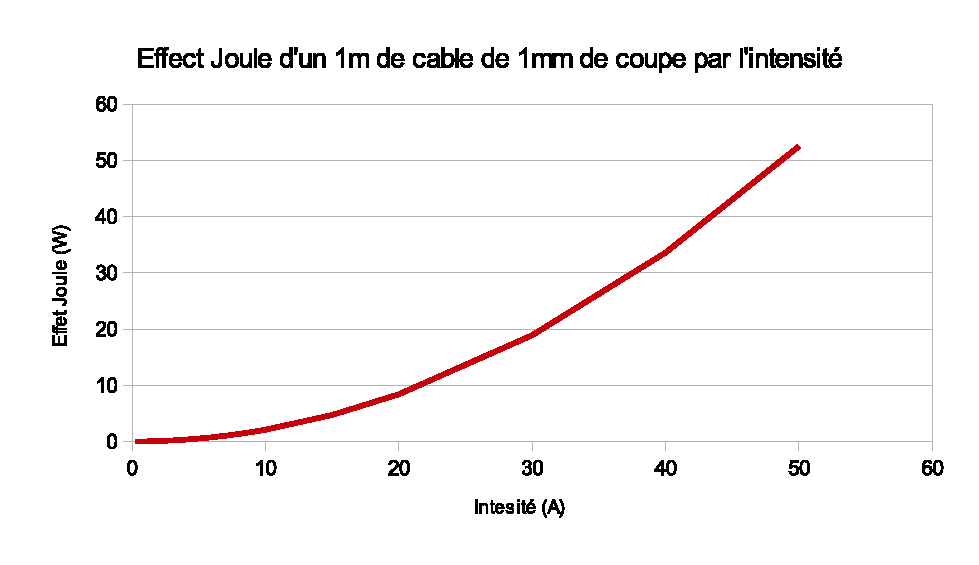
\includegraphics[width=10cm]{Joule}}
\end{center}

	Néamoins d'autres problemes peuvent occurer dans le cas d'une utilisation domstique , comme la profusion de cable qui genrent des nuisances esthetiques et des nuisances magnétiques générés par les cables nombreux qui subissent le phenomene de diaphonie (ou crosstalk), qui est une interfernce entre les signaux passant par un cable dans un cable proche. C'est d'ailleur pour cette raison que lorsque les signaux transmis sont importants et ne doivent pas etre corompus on utilise des cables torsadés qui limite le phenomene. La problematique du transport d'objets electroniques de plus en plus consomateurs mais qui se veulent autonomes se pose , ou l'on est obligé de se separer d'eux pour les recharger ceic emepechant de benficier des avantages majeurs de ces objets autonomes , avec comme exemple le cas des telephones portables , ou la problematique plus importante du rehcargement des voitures electriques qui est long , et qu'il ne faut pas oublier de brancher un cable sinon rien n'occure. Les cables electriques que nous utilisons donc depuis la création de l'electricité ne sont plus adapté a un monde qui se veut de plus en plus liberé de toute les contraintes et de s'affranchir des contraites liés au tehcnolgies filiares , avec comme exemple le devloppement des telephones portables ou 
de la wifi pour pallier la dependance cablée de l'ethernet.

\end{tabular}
\subsection{Une solution IPTS limitée : Le systeme de couplage magnetique par resonnace (CMRS)}
	Le MIT a developé en 2007 une technolgie inductive utlisant le meme pricipe que les transfomateurs electetriques ou les brosses a dent eletriques. Mais en utilisant des variations de cette tehnologies cette equipe du MIT a reussi a transmettre de l'energie a une television située de l'autre coté de la piece , assez pour l'alimenter. Mais le probleme de cette technologie est qu'elle est extremement dépendante de l'envitonement , une petite variation tel le passage d'un etre humain , un autre champ magnetique qui perturbe les syteme ou une variation de la temperature ou de l'humidité peut invalider l'experience. Cette technologie a aussi un incovenient majeur, partagé par tout les systemes inducifs de tranferts d'energie , plus souvents abregé en IPTS , qui est le rendement grandement inférieur à un cable éléctrique déployé sur la meme distance. Ceci est du a la nature meme de la technolige qui est un champ magnetique non ou peu dirigé contrairement a un cable electrique ou les eletrons n'ont que une suele direction possible pour traverser d'un bout a l'autre du systeme de transmission d'electricté.

	La depednace au conditions est du au systeme meme : il exploite la resonnace magnétique des matériaux , c'est a dire la capacité du materiau a produire une réaction energetique lorsque'il est simulé par un champ magnétique particulier , et ce "champ magnetique de resonnance" est affecté par la temperature , et il est deformé par les obstacle tel qu'un humain. Cette depedance extreme au champ magnetique est duau tres haut facteur de qualité du systeme technique utilisés dans l'experience du MIT. De plus la mise en place des bobines utilisés pour transmetre de l'electricité demande des reglages plutot complexes ou les bobines doivent etre accordées pour reagir au bon champ magnetique.
\subsection{Une solution IPTS assez fiable : Une transmission utilisant des \{Dipole coils\}}
\section{--TODO--} %Technolologie choise%
\section{Avantages et limitations de --TODO--}
\section{Technlogies alternatives pour transmetre de l'energie}

\chapter{References et sources principales}
\section{Articles scientifiques}
\section{--Et les autres trucs--}
\end{document}
